\documentclass[12pt]{article}

%packages
%\usepackage{latexsym}
\usepackage{graphicx}
\usepackage{color}
\usepackage{amsmath}
\usepackage{dsfont}
\usepackage{placeins}
\usepackage{amssymb}
\usepackage{wasysym}
\usepackage{abstract}
\usepackage{hyperref}
\usepackage{etoolbox}
\usepackage{datetime}
\usepackage{xcolor}
\usepackage{alphalph}
\settimeformat{ampmtime}

%\usepackage{pstricks,pst-node,pst-tree}

%\usepackage{algpseudocode}
%\usepackage{amsthm}
%\usepackage{hyperref}
%\usepackage{mathrsfs}
%\usepackage{amsfonts}
%\usepackage{bbding}
%\usepackage{listings}
%\usepackage{appendix}
\usepackage[margin=1in]{geometry}
%\geometry{papersize={8.5in,11in},total={6.5in,9in}}
%\usepackage{cancel}
%\usepackage{algorithmic, algorithm}

\makeatletter
\def\maxwidth{ %
  \ifdim\Gin@nat@width>\linewidth
    \linewidth
  \else
    \Gin@nat@width
  \fi
}
\makeatother

\definecolor{fgcolor}{rgb}{0.345, 0.345, 0.345}
\newcommand{\hlnum}[1]{\textcolor[rgb]{0.686,0.059,0.569}{#1}}%
\newcommand{\hlstr}[1]{\textcolor[rgb]{0.192,0.494,0.8}{#1}}%
\newcommand{\hlcom}[1]{\textcolor[rgb]{0.678,0.584,0.686}{\textit{#1}}}%
\newcommand{\hlopt}[1]{\textcolor[rgb]{0,0,0}{#1}}%
\newcommand{\hlstd}[1]{\textcolor[rgb]{0.345,0.345,0.345}{#1}}%
\newcommand{\hlkwa}[1]{\textcolor[rgb]{0.161,0.373,0.58}{\textbf{#1}}}%
\newcommand{\hlkwb}[1]{\textcolor[rgb]{0.69,0.353,0.396}{#1}}%
\newcommand{\hlkwc}[1]{\textcolor[rgb]{0.333,0.667,0.333}{#1}}%
\newcommand{\hlkwd}[1]{\textcolor[rgb]{0.737,0.353,0.396}{\textbf{#1}}}%

\usepackage{framed}
\makeatletter
\newenvironment{kframe}{%
 \def\at@end@of@kframe{}%
 \ifinner\ifhmode%
  \def\at@end@of@kframe{\end{minipage}}%
  \begin{minipage}{\columnwidth}%
 \fi\fi%
 \def\FrameCommand##1{\hskip\@totalleftmargin \hskip-\fboxsep
 \colorbox{shadecolor}{##1}\hskip-\fboxsep
     % There is no \\@totalrightmargin, so:
     \hskip-\linewidth \hskip-\@totalleftmargin \hskip\columnwidth}%
 \MakeFramed {\advance\hsize-\width
   \@totalleftmargin\z@ \linewidth\hsize
   \@setminipage}}%
 {\par\unskip\endMakeFramed%
 \at@end@of@kframe}
\makeatother

\definecolor{shadecolor}{rgb}{.77, .77, .77}
\definecolor{messagecolor}{rgb}{0, 0, 0}
\definecolor{warningcolor}{rgb}{1, 0, 1}
\definecolor{errorcolor}{rgb}{1, 0, 0}
\newenvironment{knitrout}{}{} % an empty environment to be redefined in TeX

\usepackage{alltt}
\usepackage[T1]{fontenc}

\newcommand{\qu}[1]{``#1''}
\newcounter{probnum}
\setcounter{probnum}{1}

%create definition to allow local margin changes
\def\changemargin#1#2{\list{}{\rightmargin#2\leftmargin#1}\item[]}
\let\endchangemargin=\endlist 

%allow equations to span multiple pages
\allowdisplaybreaks

%define colors and color typesetting conveniences
\definecolor{gray}{rgb}{0.5,0.5,0.5}
\definecolor{black}{rgb}{0,0,0}
\definecolor{white}{rgb}{1,1,1}
\definecolor{blue}{rgb}{0.5,0.5,1}
\newcommand{\inblue}[1]{\color{blue}#1 \color{black}}
\definecolor{green}{rgb}{0.133,0.545,0.133}
\newcommand{\ingreen}[1]{\color{green}#1 \color{black}}
\definecolor{yellow}{rgb}{1,1,0}
\newcommand{\inyellow}[1]{\color{yellow}#1 \color{black}}
\definecolor{orange}{rgb}{0.9,0.649,0}
\newcommand{\inorange}[1]{\color{orange}#1 \color{black}}
\definecolor{red}{rgb}{1,0.133,0.133}
\newcommand{\inred}[1]{\color{red}#1 \color{black}}
\definecolor{purple}{rgb}{0.58,0,0.827}
\newcommand{\inpurple}[1]{\color{purple}#1 \color{black}}
\definecolor{backgcode}{rgb}{0.97,0.97,0.8}
\definecolor{Brown}{cmyk}{0,0.81,1,0.60}
\definecolor{OliveGreen}{cmyk}{0.64,0,0.95,0.40}
\definecolor{CadetBlue}{cmyk}{0.62,0.57,0.23,0}

%define new math operators
\DeclareMathOperator*{\argmax}{arg\,max~}
\DeclareMathOperator*{\argmin}{arg\,min~}
\DeclareMathOperator*{\argsup}{arg\,sup~}
\DeclareMathOperator*{\arginf}{arg\,inf~}
\DeclareMathOperator*{\convolution}{\text{\Huge{$\ast$}}}
\newcommand{\infconv}[2]{\convolution^\infty_{#1 = 1} #2}
%true functions

%%%% GENERAL SHORTCUTS

%shortcuts for pure typesetting conveniences
\newcommand{\bv}[1]{\boldsymbol{#1}}

%shortcuts for compound constants
\newcommand{\BetaDistrConst}{\dfrac{\Gamma(\alpha + \beta)}{\Gamma(\alpha)\Gamma(\beta)}}
\newcommand{\NormDistrConst}{\dfrac{1}{\sqrt{2\pi\sigma^2}}}

%shortcuts for conventional symbols
\newcommand{\tsq}{\tau^2}
\newcommand{\tsqh}{\hat{\tau}^2}
\newcommand{\sigsq}{\sigma^2}
\newcommand{\sigsqsq}{\parens{\sigma^2}^2}
\newcommand{\sigsqovern}{\dfrac{\sigsq}{n}}
\newcommand{\tausq}{\tau^2}
\newcommand{\tausqalpha}{\tau^2_\alpha}
\newcommand{\tausqbeta}{\tau^2_\beta}
\newcommand{\tausqsigma}{\tau^2_\sigma}
\newcommand{\betasq}{\beta^2}
\newcommand{\sigsqvec}{\bv{\sigma}^2}
\newcommand{\sigsqhat}{\hat{\sigma}^2}
\newcommand{\sigsqhatmlebayes}{\sigsqhat_{\text{Bayes, MLE}}}
\newcommand{\sigsqhatmle}[1]{\sigsqhat_{#1, \text{MLE}}}
\newcommand{\bSigma}{\bv{\Sigma}}
\newcommand{\bSigmainv}{\bSigma^{-1}}
\newcommand{\thetavec}{\bv{\theta}}
\newcommand{\thetahat}{\hat{\theta}}
\newcommand{\thetahatmle}{\hat{\theta}_{\mathrm{MLE}}}
\newcommand{\thetavechatmle}{\hat{\thetavec}_{\mathrm{MLE}}}
\newcommand{\muhat}{\hat{\mu}}
\newcommand{\musq}{\mu^2}
\newcommand{\muvec}{\bv{\mu}}
\newcommand{\muhatmle}{\muhat_{\text{MLE}}}
\newcommand{\lambdahat}{\hat{\lambda}}
\newcommand{\lambdahatmle}{\lambdahat_{\text{MLE}}}
\newcommand{\etavec}{\bv{\eta}}
\newcommand{\alphavec}{\bv{\alpha}}
\newcommand{\minimaxdec}{\delta^*_{\mathrm{mm}}}
\newcommand{\ybar}{\bar{y}}
\newcommand{\xbar}{\bar{x}}
\newcommand{\Xbar}{\bar{X}}
\newcommand{\phat}{\hat{p}}
\newcommand{\Phat}{\hat{P}}
\newcommand{\Zbar}{\bar{Z}}
\newcommand{\iid}{~{\buildrel iid \over \sim}~}
\newcommand{\inddist}{~{\buildrel ind \over \sim}~}
\newcommand{\approxdist}{~{\buildrel approx \over \sim}~}
\newcommand{\equalsindist}{~{\buildrel d \over =}~}
\newcommand{\loglik}[1]{\ell\parens{#1}}
\newcommand{\thetahatkminone}{\thetahat^{(k-1)}}
\newcommand{\thetahatkplusone}{\thetahat^{(k+1)}}
\newcommand{\thetahatk}{\thetahat^{(k)}}
\newcommand{\half}{\frac{1}{2}}
\newcommand{\third}{\frac{1}{3}}
\newcommand{\twothirds}{\frac{2}{3}}
\newcommand{\fourth}{\frac{1}{4}}
\newcommand{\fifth}{\frac{1}{5}}
\newcommand{\sixth}{\frac{1}{6}}

%shortcuts for vector and matrix notation
\newcommand{\A}{\bv{A}}
\newcommand{\At}{\A^T}
\newcommand{\Ainv}{\inverse{\A}}
\newcommand{\B}{\bv{B}}
\newcommand{\K}{\bv{K}}
\newcommand{\Kt}{\K^T}
\newcommand{\Kinv}{\inverse{K}}
\newcommand{\Kinvt}{(\Kinv)^T}
\newcommand{\M}{\bv{M}}
\newcommand{\Bt}{\B^T}
\newcommand{\Q}{\bv{Q}}
\newcommand{\Qt}{\Q^T}
\newcommand{\R}{\bv{R}}
\newcommand{\Rt}{\R^T}
\newcommand{\Z}{\bv{Z}}
\newcommand{\X}{\bv{X}}
\newcommand{\Xsub}{\X_{\text{(sub)}}}
\newcommand{\Xsubadj}{\X_{\text{(sub,adj)}}}
\newcommand{\I}{\bv{I}}
\newcommand{\Y}{\bv{Y}}
\newcommand{\sigsqI}{\sigsq\I}
\renewcommand{\P}{\bv{P}}
\newcommand{\Psub}{\P_{\text{(sub)}}}
\newcommand{\Pt}{\P^T}
\newcommand{\Pii}{P_{ii}}
\newcommand{\Pij}{P_{ij}}
\newcommand{\IminP}{(\I-\P)}
\newcommand{\Xt}{\bv{X}^T}
\newcommand{\XtX}{\Xt\X}
\newcommand{\XtXinv}{\parens{\Xt\X}^{-1}}
\newcommand{\XtXinvXt}{\XtXinv\Xt}
\newcommand{\XXtXinvXt}{\X\XtXinvXt}
\newcommand{\x}{\bv{x}}
\renewcommand{\b}{\bv{b}}
\newcommand{\onevec}{\bv{1}}
\newcommand{\oneton}{1, \ldots, n}
\newcommand{\yoneton}{y_1, \ldots, y_n}
\newcommand{\yonetonorder}{y_{(1)}, \ldots, y_{(n)}}
\newcommand{\Yoneton}{Y_1, \ldots, Y_n}
\newcommand{\iinoneton}{i \in \braces{\oneton}}
\newcommand{\onetom}{1, \ldots, m}
\newcommand{\jinonetom}{j \in \braces{\onetom}}
\newcommand{\xoneton}{x_1, \ldots, x_n}
\newcommand{\Xoneton}{X_1, \ldots, X_n}
\newcommand{\xt}{\x^T}
\newcommand{\y}{\bv{y}}
\newcommand{\yt}{\y^T}
\renewcommand{\c}{\bv{c}}
\newcommand{\ct}{\c^T}
\newcommand{\tstar}{\bv{t}^*}
\renewcommand{\u}{\bv{u}}
\renewcommand{\v}{\bv{v}}
\renewcommand{\a}{\bv{a}}
\newcommand{\s}{\bv{s}}
\newcommand{\yadj}{\y_{\text{(adj)}}}
\newcommand{\xjadj}{\x_{j\text{(adj)}}}
\newcommand{\xjadjM}{\x_{j \perp M}}
\newcommand{\yhat}{\hat{\y}}
\newcommand{\yhatsub}{\yhat_{\text{(sub)}}}
\newcommand{\yhatstar}{\yhat^*}
\newcommand{\yhatstarnew}{\yhatstar_{\text{new}}}
\newcommand{\z}{\bv{z}}
\newcommand{\zt}{\z^T}
\newcommand{\bb}{\bv{b}}
\newcommand{\bbt}{\bb^T}
\newcommand{\bbeta}{\bv{\beta}}
\newcommand{\beps}{\bv{\epsilon}}
\newcommand{\bepst}{\beps^T}
\newcommand{\e}{\bv{e}}
\newcommand{\Mofy}{\M(\y)}
\newcommand{\KofAlpha}{K(\alpha)}
\newcommand{\ellset}{\mathcal{L}}
\newcommand{\oneminalph}{1-\alpha}
\newcommand{\SSE}{\text{SSE}}
\newcommand{\SSEsub}{\text{SSE}_{\text{(sub)}}}
\newcommand{\MSE}{\text{MSE}}
\newcommand{\RMSE}{\text{RMSE}}
\newcommand{\SSR}{\text{SSR}}
\newcommand{\SST}{\text{SST}}
\newcommand{\JSest}{\delta_{\text{JS}}(\x)}
\newcommand{\Bayesest}{\delta_{\text{Bayes}}(\x)}
\newcommand{\EmpBayesest}{\delta_{\text{EmpBayes}}(\x)}
\newcommand{\BLUPest}{\delta_{\text{BLUP}}}
\newcommand{\MLEest}[1]{\hat{#1}_{\text{MLE}}}

%shortcuts for Linear Algebra stuff (i.e. vectors and matrices)
\newcommand{\twovec}[2]{\bracks{\begin{array}{c} #1 \\ #2 \end{array}}}
\newcommand{\threevec}[3]{\bracks{\begin{array}{c} #1 \\ #2 \\ #3 \end{array}}}
\newcommand{\fivevec}[5]{\bracks{\begin{array}{c} #1 \\ #2 \\ #3 \\ #4 \\ #5 \end{array}}}
\newcommand{\twobytwomat}[4]{\bracks{\begin{array}{cc} #1 & #2 \\ #3 & #4 \end{array}}}
\newcommand{\threebytwomat}[6]{\bracks{\begin{array}{cc} #1 & #2 \\ #3 & #4 \\ #5 & #6 \end{array}}}

%shortcuts for conventional compound symbols
\newcommand{\thetainthetas}{\theta \in \Theta}
\newcommand{\reals}{\mathbb{R}}
\newcommand{\complexes}{\mathbb{C}}
\newcommand{\rationals}{\mathbb{Q}}
\newcommand{\integers}{\mathbb{Z}}
\newcommand{\naturals}{\mathbb{N}}
\newcommand{\forallninN}{~~\forall n \in \naturals}
\newcommand{\forallxinN}[1]{~~\forall #1 \in \reals}
\newcommand{\matrixdims}[2]{\in \reals^{\,#1 \times #2}}
\newcommand{\inRn}[1]{\in \reals^{\,#1}}
\newcommand{\mathimplies}{\quad\Rightarrow\quad}
\newcommand{\mathlogicequiv}{\quad\Leftrightarrow\quad}
\newcommand{\eqncomment}[1]{\quad \text{(#1)}}
\newcommand{\limitn}{\lim_{n \rightarrow \infty}}
\newcommand{\limitN}{\lim_{N \rightarrow \infty}}
\newcommand{\limitd}{\lim_{d \rightarrow \infty}}
\newcommand{\limitt}{\lim_{t \rightarrow \infty}}
\newcommand{\limitsupn}{\limsup_{n \rightarrow \infty}~}
\newcommand{\limitinfn}{\liminf_{n \rightarrow \infty}~}
\newcommand{\limitk}{\lim_{k \rightarrow \infty}}
\newcommand{\limsupn}{\limsup_{n \rightarrow \infty}}
\newcommand{\limsupk}{\limsup_{k \rightarrow \infty}}
\newcommand{\floor}[1]{\left\lfloor #1 \right\rfloor}
\newcommand{\ceil}[1]{\left\lceil #1 \right\rceil}

%shortcuts for environments
\newcommand{\beqn}{\vspace{-0.25cm}\begin{eqnarray*}}
\newcommand{\eeqn}{\end{eqnarray*}}
\newcommand{\bneqn}{\vspace{-0.25cm}\begin{eqnarray}}
\newcommand{\eneqn}{\end{eqnarray}}

%shortcuts for mini environments
\newcommand{\parens}[1]{\left(#1\right)}
\newcommand{\squared}[1]{\parens{#1}^2}
\newcommand{\tothepow}[2]{\parens{#1}^{#2}}
\newcommand{\prob}[1]{\mathbb{P}\parens{#1}}
\newcommand{\cprob}[2]{\prob{#1~|~#2}}
\newcommand{\littleo}[1]{o\parens{#1}}
\newcommand{\bigo}[1]{O\parens{#1}}
\newcommand{\Lp}[1]{\mathbb{L}^{#1}}
\renewcommand{\arcsin}[1]{\text{arcsin}\parens{#1}}
\newcommand{\prodonen}[2]{\bracks{\prod_{#1=1}^n #2}}
\newcommand{\mysum}[4]{\sum_{#1=#2}^{#3} #4}
\newcommand{\sumonen}[2]{\sum_{#1=1}^n #2}
\newcommand{\infsum}[2]{\sum_{#1=1}^\infty #2}
\newcommand{\infprod}[2]{\prod_{#1=1}^\infty #2}
\newcommand{\infunion}[2]{\bigcup_{#1=1}^\infty #2}
\newcommand{\infinter}[2]{\bigcap_{#1=1}^\infty #2}
\newcommand{\infintegral}[2]{\int^\infty_{-\infty} #2 ~\text{d}#1}
\newcommand{\supthetas}[1]{\sup_{\thetainthetas}\braces{#1}}
\newcommand{\bracks}[1]{\left[#1\right]}
\newcommand{\braces}[1]{\left\{#1\right\}}
\newcommand{\set}[1]{\left\{#1\right\}}
\newcommand{\abss}[1]{\left|#1\right|}
\newcommand{\norm}[1]{\left|\left|#1\right|\right|}
\newcommand{\normsq}[1]{\norm{#1}^2}
\newcommand{\inverse}[1]{\parens{#1}^{-1}}
\newcommand{\rowof}[2]{\parens{#1}_{#2\cdot}}

%shortcuts for functionals
\newcommand{\realcomp}[1]{\text{Re}\bracks{#1}}
\newcommand{\imagcomp}[1]{\text{Im}\bracks{#1}}
\newcommand{\range}[1]{\text{range}\bracks{#1}}
\newcommand{\colsp}[1]{\text{colsp}\bracks{#1}}
\newcommand{\rowsp}[1]{\text{rowsp}\bracks{#1}}
\newcommand{\tr}[1]{\text{tr}\bracks{#1}}
\newcommand{\rank}[1]{\text{rank}\bracks{#1}}
\newcommand{\proj}[2]{\text{Proj}_{#1}\bracks{#2}}
\newcommand{\projcolspX}[1]{\text{Proj}_{\colsp{\X}}\bracks{#1}}
\newcommand{\median}[1]{\text{median}\bracks{#1}}
\newcommand{\mean}[1]{\text{mean}\bracks{#1}}
\newcommand{\dime}[1]{\text{dim}\bracks{#1}}
\renewcommand{\det}[1]{\text{det}\bracks{#1}}
\newcommand{\expe}[1]{\mathbb{E}\bracks{#1}}
\newcommand{\expeabs}[1]{\expe{\abss{#1}}}
\newcommand{\expesub}[2]{\mathbb{E}_{#1}\bracks{#2}}
\newcommand{\indic}[1]{\mathds{1}_{#1}}
\newcommand{\var}[1]{\mathbb{V}\text{ar}\bracks{#1}}
\newcommand{\cov}[2]{\mathbb{C}\text{ov}\bracks{#1, #2}}
\newcommand{\corr}[2]{\text{Corr}\bracks{#1, #2}}
\newcommand{\se}[1]{\mathbb{S}\text{E}\bracks{#1}}
\newcommand{\seest}[1]{\hat{\mathbb{S}\text{E}}\bracks{#1}}
\newcommand{\bias}[1]{\text{Bias}\bracks{#1}}
\newcommand{\derivop}[2]{\dfrac{\text{d}}{\text{d} #1}\bracks{#2}}
\newcommand{\partialop}[2]{\dfrac{\partial}{\partial #1}\bracks{#2}}
\newcommand{\secpartialop}[2]{\dfrac{\partial^2}{\partial #1^2}\bracks{#2}}
\newcommand{\mixpartialop}[3]{\dfrac{\partial^2}{\partial #1 \partial #2}\bracks{#3}}

%shortcuts for functions
\renewcommand{\exp}[1]{\mathrm{exp}\parens{#1}}
\renewcommand{\cos}[1]{\text{cos}\parens{#1}}
\renewcommand{\sin}[1]{\text{sin}\parens{#1}}
\newcommand{\sign}[1]{\text{sign}\parens{#1}}
\newcommand{\are}[1]{\mathrm{ARE}\parens{#1}}
\newcommand{\natlog}[1]{\ln\parens{#1}}
\newcommand{\oneover}[1]{\frac{1}{#1}}
\newcommand{\overtwo}[1]{\frac{#1}{2}}
\newcommand{\overn}[1]{\frac{#1}{n}}
\newcommand{\oneoversqrt}[1]{\oneover{\sqrt{#1}}}
\newcommand{\sqd}[1]{\parens{#1}^2}
\newcommand{\loss}[1]{\ell\parens{\theta, #1}}
\newcommand{\losstwo}[2]{\ell\parens{#1, #2}}
\newcommand{\cf}{\phi(t)}

%English language specific shortcuts
\newcommand{\ie}{\textit{i.e.} }
\newcommand{\AKA}{\textit{AKA} }
\renewcommand{\iff}{\textit{iff}}
\newcommand{\eg}{\textit{e.g.} }
\newcommand{\st}{\textit{s.t.} }
\newcommand{\wrt}{\textit{w.r.t.} }
\newcommand{\mathst}{~~\text{\st}~~}
\newcommand{\mathand}{~~\text{and}~~}
\newcommand{\ala}{\textit{a la} }
\newcommand{\ppp}{posterior predictive p-value}
\newcommand{\dd}{dataset-to-dataset}

%shortcuts for distribution titles
\newcommand{\logistic}[2]{\mathrm{Logistic}\parens{#1,\,#2}}
\newcommand{\bernoulli}[1]{\mathrm{Bernoulli}\parens{#1}}
\newcommand{\betanot}[2]{\mathrm{Beta}\parens{#1,\,#2}}
\newcommand{\stdbetanot}{\betanot{\alpha}{\beta}}
\newcommand{\multnormnot}[3]{\mathcal{N}_{#1}\parens{#2,\,#3}}
\newcommand{\normnot}[2]{\mathcal{N}\parens{#1,\,#2}}
\newcommand{\classicnormnot}{\normnot{\mu}{\sigsq}}
\newcommand{\stdnormnot}{\normnot{0}{1}}
\newcommand{\uniformdiscrete}[1]{\mathrm{Uniform}\parens{\braces{#1}}}
\newcommand{\uniform}[2]{\mathrm{U}\parens{#1,\,#2}}
\newcommand{\stduniform}{\uniform{0}{1}}
\newcommand{\geometric}[1]{\mathrm{Geometric}\parens{#1}}
\newcommand{\hypergeometric}[3]{\mathrm{Hypergeometric}\parens{#1,\,#2,\,#3}}
\newcommand{\exponential}[1]{\mathrm{Exp}\parens{#1}}
\newcommand{\gammadist}[2]{\mathrm{Gamma}\parens{#1, #2}}
\newcommand{\poisson}[1]{\mathrm{Poisson}\parens{#1}}
\newcommand{\binomial}[2]{\mathrm{Binomial}\parens{#1,\,#2}}
\newcommand{\negbin}[2]{\mathrm{NegBin}\parens{#1,\,#2}}
\newcommand{\rayleigh}[1]{\mathrm{Rayleigh}\parens{#1}}
\newcommand{\multinomial}[2]{\mathrm{Multinomial}\parens{#1,\,#2}}
\newcommand{\gammanot}[2]{\mathrm{Gamma}\parens{#1,\,#2}}
\newcommand{\cauchynot}[2]{\text{Cauchy}\parens{#1,\,#2}}
\newcommand{\invchisqnot}[1]{\text{Inv}\chisq{#1}}
\newcommand{\invscaledchisqnot}[2]{\text{ScaledInv}\ncchisq{#1}{#2}}
\newcommand{\invgammanot}[2]{\text{InvGamma}\parens{#1,\,#2}}
\newcommand{\chisq}[1]{\chi^2_{#1}}
\newcommand{\ncchisq}[2]{\chi^2_{#1}\parens{#2}}
\newcommand{\ncF}[3]{F_{#1,#2}\parens{#3}}

%shortcuts for PDF's of common distributions
\newcommand{\logisticpdf}[3]{\oneover{#3}\dfrac{\exp{-\dfrac{#1 - #2}{#3}}}{\parens{1+\exp{-\dfrac{#1 - #2}{#3}}}^2}}
\newcommand{\betapdf}[3]{\dfrac{\Gamma(#2 + #3)}{\Gamma(#2)\Gamma(#3)}#1^{#2-1} (1-#1)^{#3-1}}
\newcommand{\normpdf}[3]{\frac{1}{\sqrt{2\pi#3}}\exp{-\frac{1}{2#3}(#1 - #2)^2}}
\newcommand{\normpdfvarone}[2]{\dfrac{1}{\sqrt{2\pi}}e^{-\half(#1 - #2)^2}}
\newcommand{\chisqpdf}[2]{\dfrac{1}{2^{#2/2}\Gamma(#2/2)}\; {#1}^{#2/2-1} e^{-#1/2}}
\newcommand{\invchisqpdf}[2]{\dfrac{2^{-\overtwo{#1}}}{\Gamma(#2/2)}\,{#1}^{-\overtwo{#2}-1}  e^{-\oneover{2 #1}}}
\newcommand{\exponentialpdf}[2]{#2\exp{-#2#1}}
\newcommand{\poissonpdf}[2]{\dfrac{e^{-#1} #1^{#2}}{#2!}}
\newcommand{\binomialpdf}[3]{\binom{#2}{#1}#3^{#1}(1-#3)^{#2-#1}}
\newcommand{\rayleighpdf}[2]{\dfrac{#1}{#2^2}\exp{-\dfrac{#1^2}{2 #2^2}}}
\newcommand{\gammapdf}[3]{\dfrac{#3^#2}{\Gamma\parens{#2}}#1^{#2-1}\exp{-#3 #1}}
\newcommand{\cauchypdf}[3]{\oneover{\pi} \dfrac{#3}{\parens{#1-#2}^2 + #3^2}}
\newcommand{\Gammaf}[1]{\Gamma\parens{#1}}

%shortcuts for miscellaneous typesetting conveniences
\newcommand{\notesref}[1]{\marginpar{\color{gray}\tt #1\color{black}}}

%%%% DOMAIN-SPECIFIC SHORTCUTS

%Real analysis related shortcuts
\newcommand{\zeroonecl}{\bracks{0,1}}
\newcommand{\forallepsgrzero}{\forall \epsilon > 0~~}
\newcommand{\lessthaneps}{< \epsilon}
\newcommand{\fraccomp}[1]{\text{frac}\bracks{#1}}

%Bayesian related shortcuts
\newcommand{\yrep}{y^{\text{rep}}}
\newcommand{\yrepisq}{(\yrep_i)^2}
\newcommand{\yrepvec}{\bv{y}^{\text{rep}}}


%Probability shortcuts
\newcommand{\SigField}{\mathcal{F}}
\newcommand{\ProbMap}{\mathcal{P}}
\newcommand{\probtrinity}{\parens{\Omega, \SigField, \ProbMap}}
\newcommand{\convp}{~{\buildrel p \over \rightarrow}~}
\newcommand{\convLp}[1]{~{\buildrel \Lp{#1} \over \rightarrow}~}
\newcommand{\nconvp}{~{\buildrel p \over \nrightarrow}~}
\newcommand{\convae}{~{\buildrel a.e. \over \longrightarrow}~}
\newcommand{\convau}{~{\buildrel a.u. \over \longrightarrow}~}
\newcommand{\nconvau}{~{\buildrel a.u. \over \nrightarrow}~}
\newcommand{\nconvae}{~{\buildrel a.e. \over \nrightarrow}~}
\newcommand{\convd}{~{\buildrel \mathcal{D} \over \rightarrow}~}
\newcommand{\nconvd}{~{\buildrel \mathcal{D} \over \nrightarrow}~}
\newcommand{\withprob}{~~\text{w.p.}~~}
\newcommand{\io}{~~\text{i.o.}}

\newcommand{\Acl}{\bar{A}}
\newcommand{\ENcl}{\bar{E}_N}
\newcommand{\diam}[1]{\text{diam}\parens{#1}}

\newcommand{\taua}{\tau_a}

\newcommand{\myint}[4]{\int_{#2}^{#3} #4 \,\text{d}#1}
\newcommand{\laplacet}[1]{\mathscr{L}\bracks{#1}}
\newcommand{\laplaceinvt}[1]{\mathscr{L}^{-1}\bracks{#1}}
\renewcommand{\min}[1]{\text{min}\braces{#1}}
\renewcommand{\max}[1]{\text{max}\braces{#1}}

\newcommand{\Vbar}[1]{\bar{V}\parens{#1}}
\newcommand{\expnegrtau}{\exp{-r\tau}}

%%% problem typesetting
\definecolor{darkgrey}{rgb}{0.10,0.10,0.9}

\newcommand{\problem}[1]{\noindent \colorbox{black}{{\color{yellow} \large{\textsf{\textbf{Problem \arabic{probnum}}}}~}} \addtocounter{probnum}{1} \vspace{0.2cm} \\ \iftoggle{professormode}{}{\color{darkgrey}} #1}

\newcommand{\easysubproblem}[1]{\ingreen{\item} \iftoggle{professormode}{}{\color{darkgrey}} [easy] #1 \color{black} }
\newcommand{\intermediatesubproblem}[1]{\inorange{\item} \iftoggle{professormode}{}{\color{darkgrey}} [harder] #1 \color{black} }
\newcommand{\hardsubproblem}[1]{\inred{\item} \iftoggle{professormode}{}{\color{darkgrey}} [difficult] #1 \color{black} }
\newcommand{\extracreditsubproblem}[1]{\inpurple{\item} \iftoggle{professormode}{}{\color{darkgrey}} [E.C.] #1 \color{black} }


\newcommand{\spc}[1]{\iftoggle{professormode}{\\ \vspace{#1cm}}{\\ \vspace{-0.3cm}}}

\makeatletter
\newalphalph{\alphmult}[mult]{\@alph}{26}
\renewcommand{\labelenumi}{(\alphmult{\value{enumi}})}

\newcommand{\support}[1]{\text{Supp}\bracks{#1}}
\newcommand{\mode}[1]{\text{Mode}\bracks{#1}}
\newcommand{\IQR}[1]{\text{IQR}\bracks{#1}}
\newcommand{\quantile}[2]{\text{Quantile}\bracks{#1,\,#2}}


\newtoggle{professormode}



\title{MATH 342W / 650.4 / RM742 Spring \the\year~HW \#1}

\author{Mohammed Hasan} %STUDENTS: Mohammed Hasan

\iftoggle{professormode}{
\date{Due 11:59PM Thursday, February 10, \the\year~by email \\ \vspace{0.5cm} \small (this document last updated \currenttime~on \today)}
}

\renewcommand{\abstractname}{Instructions and Philosophy}

\begin{document}
\maketitle

\iftoggle{professormode}{
\begin{abstract}
The path to success in this class is to do many problems. Unlike other courses, exclusively doing reading(s) will not help. Coming to lecture is akin to watching workout videos; thinking about and solving problems on your own is the actual ``working out.''  Feel free to \qu{work out} with others; \textbf{I want you to work on this in groups.}

Reading is still \textit{required}. For this homework set, read the first chapter of \qu{Learning from Data} and the introduction and Chapter 1 of Silver's book. Of course, you should be googling and reading about all the concepts introduced in class online. This is your responsibility to supplement in-class with your own readings.

The problems below are color coded: \ingreen{green} problems are considered \textit{easy} and marked \qu{[easy]}; \inorange{yellow} problems are considered \textit{intermediate} and marked \qu{[harder]}, \inred{red} problems are considered \textit{difficult} and marked \qu{[difficult]} and \inpurple{purple} problems are extra credit. The \textit{easy} problems are intended to be ``giveaways'' if you went to class. Do as much as you can of the others; I expect you to at least attempt the \textit{difficult} problems. 

This homework is worth 100 points but the point distribution will not be determined until after the due date. See syllabus for the policy on late homework.

Up to 7 points are given as a bonus if the homework is typed using \LaTeX. Links to instaling \LaTeX~and program for compiling \LaTeX~is found on the syllabus. You are encouraged to use \url{overleaf.com}. If you are handing in homework this way, read the comments in the code; there are two lines to comment out and you should replace my name with yours and write your section. The easiest way to use overleaf is to copy the raw text from hwxx.tex and preamble.tex into two new overleaf tex files with the same name. If you are asked to make drawings, you can take a picture of your handwritten drawing and insert them as figures or leave space using the \qu{$\backslash$vspace} command and draw them in after printing or attach them stapled.

The document is available with spaces for you to write your answers. If not using \LaTeX, print this document and write in your answers. I do not accept homeworks which are \textit{not} on this printout. Keep this first page printed for your records.

\end{abstract}

\thispagestyle{empty}
\vspace{1cm}
NAME: \line(1,0){380}
\clearpage
}

\problem{These are questions about Silver's book, the introduction and chapter 1.}

\begin{enumerate}

\easysubproblem{What is the difference between \emph{predict} and \emph{forecast}? Are these two terms used interchangably today?}\spc{4}

The terms \emph{predict} and \emph{forecast} are used interchangably today despite there being clear differences between the two during shakespearian times
\begin{itemize}
  \item \emph{forecast} : means to plan under conditions of uncertainty
  \item \emph{predict} : is described as "what the soothersayer told you" meaning it is certain
\end{itemize}

\easysubproblem{What is John P. Ioannidis's findings and what are its implications?}\spc{5}

John P. Ioannidis's findings detailed in the paper titled "why most published Research Findings are False" says that a significant portion of positive findings in biomedical research journals are not able to be applied to real-world settings. The implications of his findings are that it questions the reliability of the research. Bayer laboratories confirmed his hypothesis.

\easysubproblem{What are the human being's most powerful defense (according to Silver)? Answer using the language from class.}\spc{4}

Human beings most powerful defense is their ability to recognize patterns.

\easysubproblem{Information is increasing at a rapid pace, but what is not increasing?}\spc{3}

Our human ability to process information is getting outpaced by the information that is increasing.

\hardsubproblem{Silver admits that we will always be subjectively biased when making predictions. However, he believes there is an objective truth. In class, how did we describe the objective truth? Answer using notation from class i.e. $t,f, g, h^*, \delta, \epsilon, t, z_1, \ldots, z_t, \delta, \mathbb{D}$, $\mathcal{H}, \mathcal{A}, \mathcal{X}, \mathcal{Y}, X, y, n, p$, $x_{\cdot 1}, \ldots, x_{\cdot p}, x_{1 \cdot}, \ldots, x_{n \cdot}$, etc.}\spc{3}

I believe the objective truth is: $y = t(z_1, \ldots, z_t)$ where $y$ is the response/dependent variable and the $z$'s are the proximal causes which the unknown function, $t$, uses to obtain.

\easysubproblem{In a nutshell, what is Karl Popper's (a famous philosopher of science) definition of \emph{science}?}\spc{4}

Popper's definition of science relies on the idea of falsifiable. For him, a hypothesis is only scientific when it can be proven through real-world experimentation.

\intermediatesubproblem{Why did the ratings agencies say the probability of a CDO defaulting was 0.12\% instead of the 28\% that actually occured? Answer using concepts from class.}\spc{4}

The models that the rating agencies used were flawed and the agencies were relying on them heavily. 
pg38 "forecasting models were full of faulty assumptions and false confidence about the risk."

\easysubproblem{What is the difference between \emph{risk} and \emph{uncertainty} according to Silver's definitions?}\spc{4}

\begin{itemize}
  \item \emph{Risk} : can be evaluated numerically such as a price.
  \item \emph{Uncertainty} : is harder to measure since it can not be defined numerically.
\end{itemize}

\hardsubproblem{How does Silver define \emph{out of sample}? Answer using notation from class i.e. $t,f, g, h^*, \delta, \epsilon, z_1, \ldots, z_t, \delta, \mathbb{D}, \mathcal{H}, \mathcal{A}, \mathcal{X}, \mathcal{Y}, X, y, n, p, x_{\cdot 1}, \ldots, x_{\cdot p}, x_{1 \cdot}, \ldots, x_{n \cdot}$, etc. WARNING: Silver defines \emph{out of sample} completely differently than the literature, than practitioners in industry and how we will define it in class in a month or so. We will explore what he is talking about in class in the future and we will term this concept differently, using the more widely accepted terminology. So please forget the phrase \emph{out of sample} for now as we will introduce it later in class as something else. There will be other such terms in his book and I will provide this disclaimer at these appropriate times.}\spc{7}

Silver defines \emph{out of sample} by giving an example of driving under the influence. Your problem is \emph{out of sample} when you are using an X that is irrelevant. Your car trips driven sober should not be counted if you are driving drunk. This would be your first time driving drunk.

\intermediatesubproblem{Look up \emph{bias} and \emph{variance} online or in a statistics textbook. Connect these concepts to Silver's terms \emph{accuracy} and \emph{precision}. This is another example of Silver using non-standard terminology.}\spc{9}

\emph{bias} and \emph{variance} are very similar to \emph{accuracy} and \emph{precision}. \emph{accuracy} is the ability to land closer to the "Truth" which is the inversion of \emph{bias} \\
\\
High accuracy = Low Bias \\
\\
\emph{precision} is the range of the cluster. If the cluster is further apart it has Low Precision \\
\\
High Precision = Low Variance

\end{enumerate}


\problem{Below are some questions about the theory of modeling.}

\begin{enumerate}

\easysubproblem{Redraw the illustration of Earth and the table-top globe except do not use the Earth and a table-top globe as examples (use another example). The quadrants are connected with arrows. Label these arrows appropriately.}\spc{11}

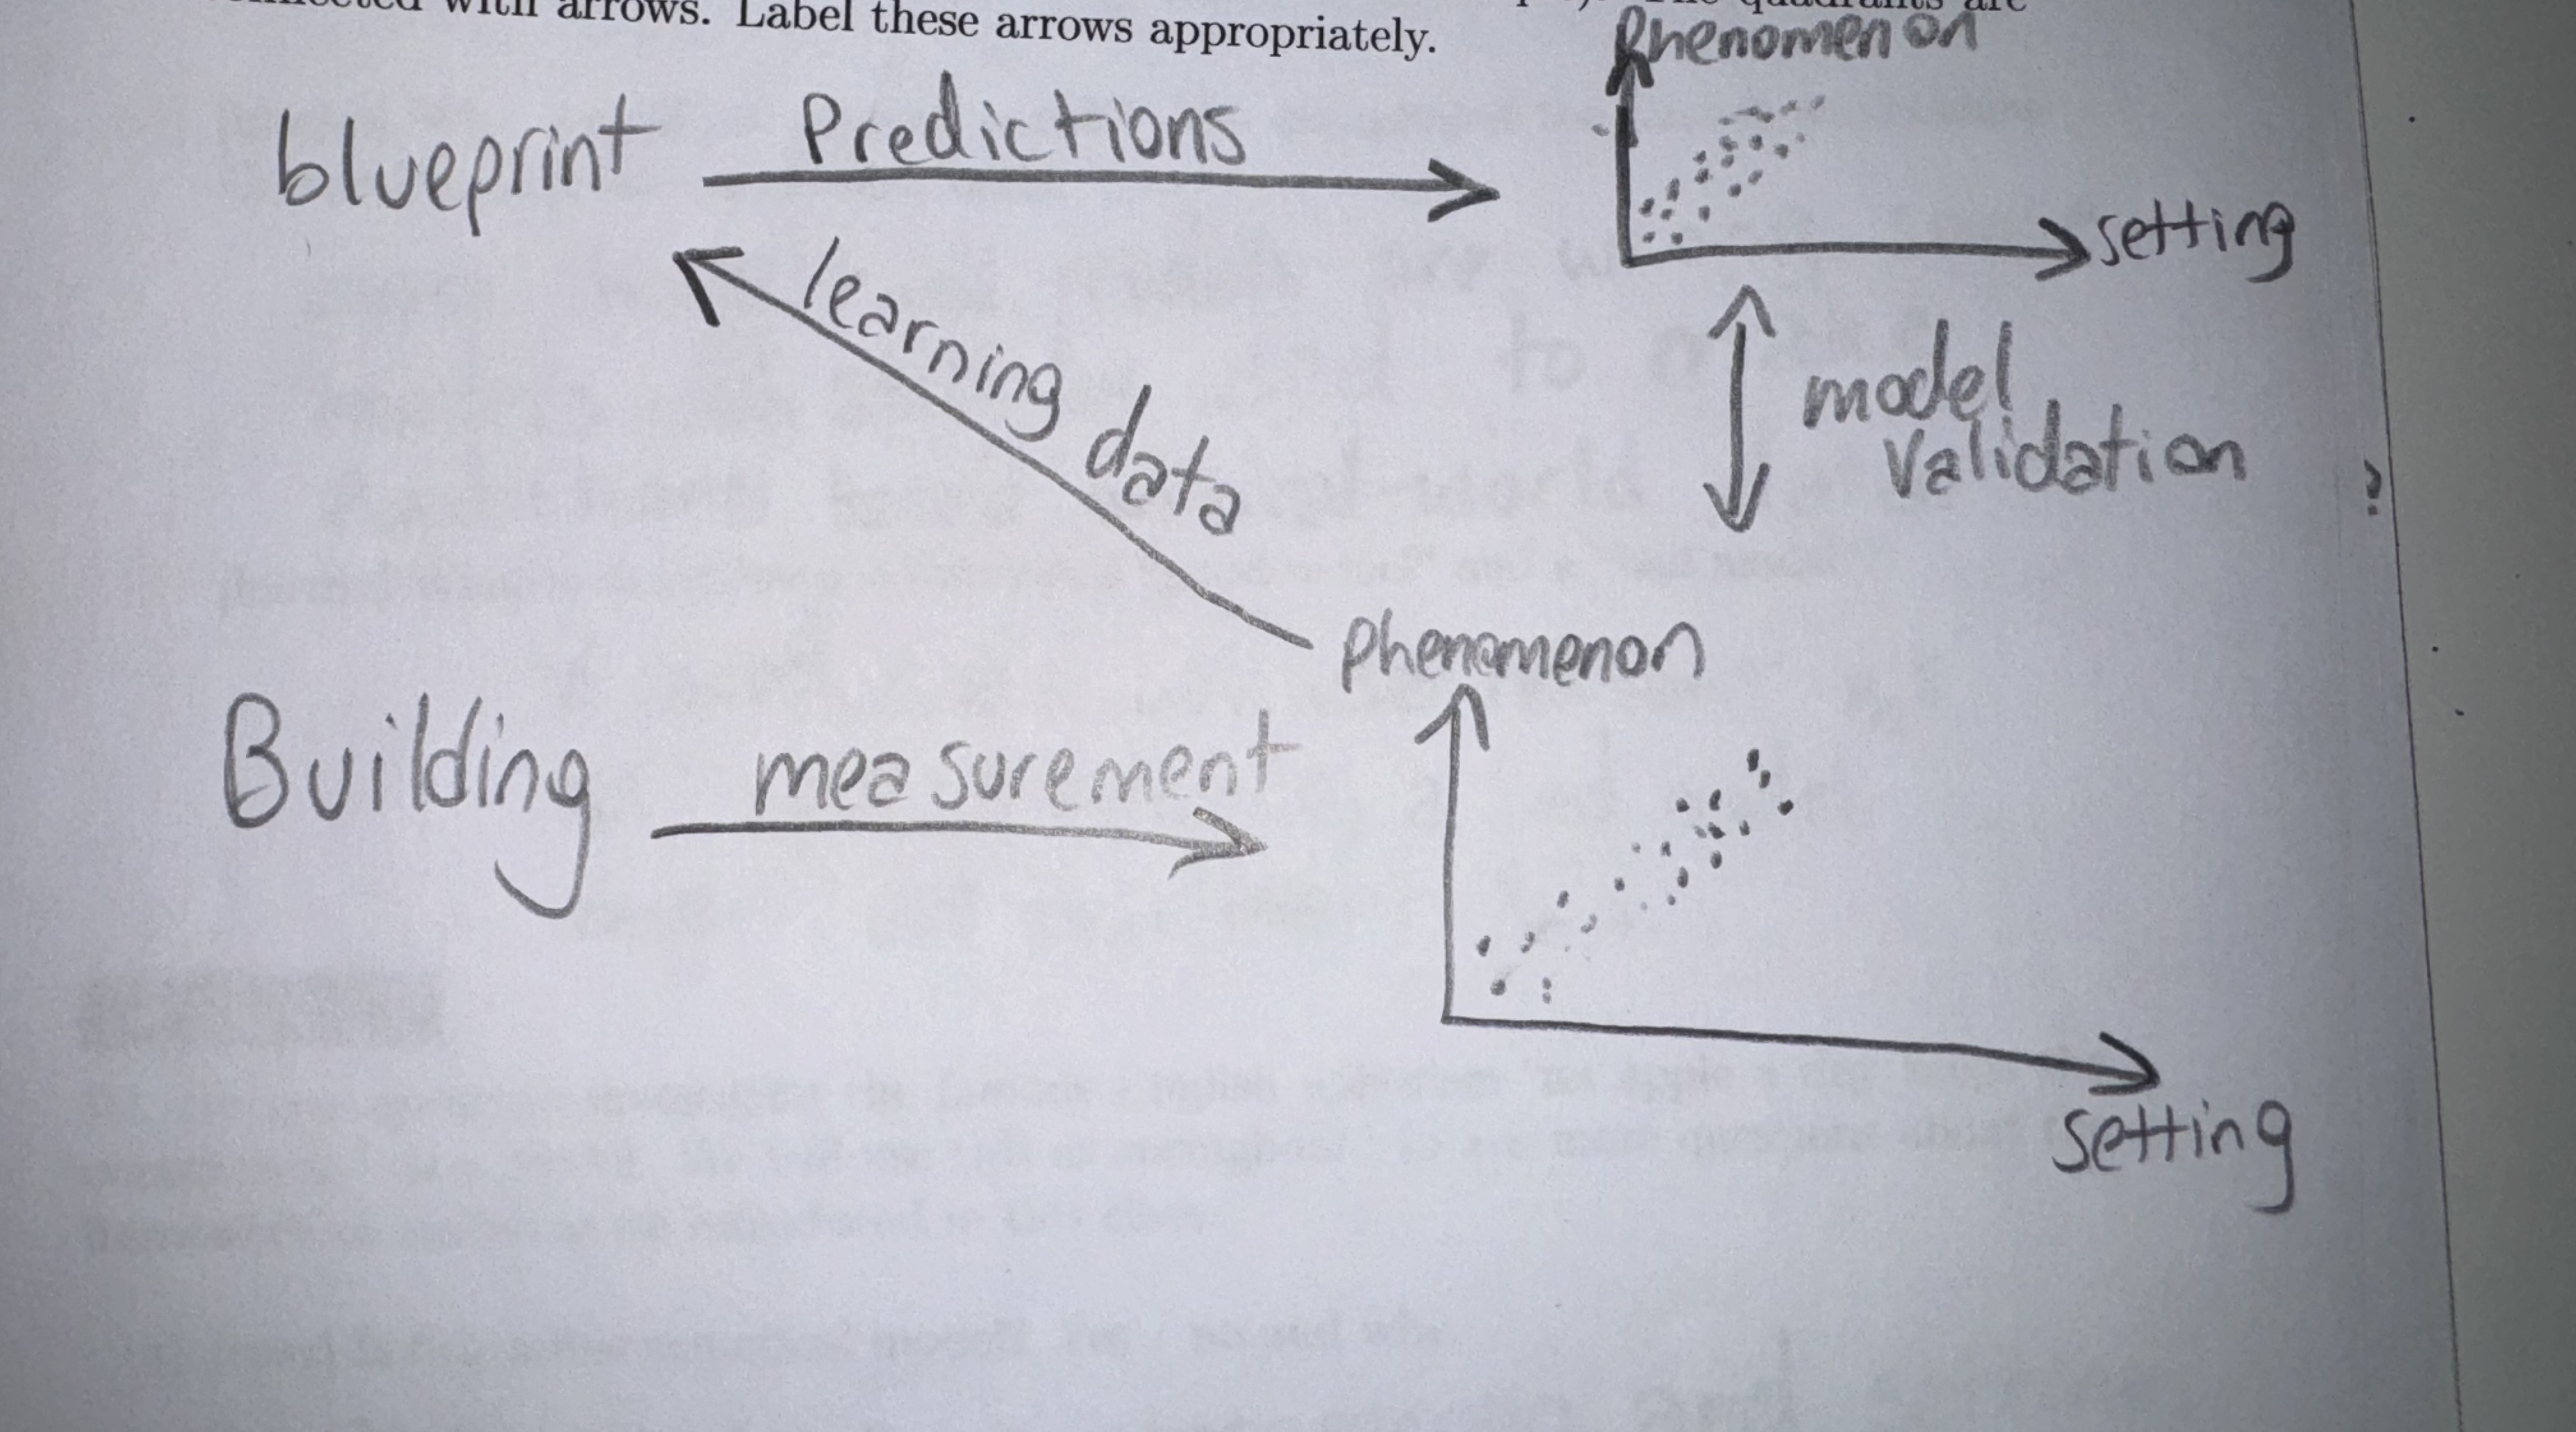
\includegraphics[scale=0.1]{IMG_4462.jpg}


\easysubproblem{Pursuant to the fix in the previous question, how do we define \emph{data} for the purposes of this class?}\spc{2}

\emph{Data}, for this class, pertains to results of events that already occured that can be used to predict the outcome of another event.

\easysubproblem{Pursuant to the fix in the previous question, how do we define \emph{predictions} for the purposes of this class?}\spc{3}

According to our illustration, \emph{Predictions} are expected calculations which we derive by interpretting the real world phenomenon.

\easysubproblem{Why are \qu{all models wrong}? We are quoting the famous statisticians George Box and Norman Draper here.}\spc{2}

\qu{all models wrong} because they are not fully accurate and precise.

\intermediatesubproblem{Why are \qu{[some models] useful}? We are quoting the famous statisticians George Box and Norman Draper here.}\spc{2}

Even though all models are wrong, some models can still be used to make predictions based on real-world data.

\intermediatesubproblem{What is the difference between a "good model" and a "bad model"?}\spc{2}

\end{enumerate}




\problem{We are now going to investigate the famous English aphorism \qu{an apple a day keeps the doctor away} as a model. We will use this as springboard to ask more questions about the framework of modeling we introduced in this class.}

\begin{enumerate}


\easysubproblem{Is this a mathematical model? Yes / no and why.}\spc{3}

Yes, we have a phenomenon and setting, we can also used metrics to measure them.

\easysubproblem{What is(are) the input(s) in this model?}\spc{3}

1 apple

\easysubproblem{What is(are) the output(s) in this model?}\spc{3}

Doctor away

\intermediatesubproblem{How good / bad do you think this model is and why?}\spc{3}

I believe, although it encourages a healthy lifestyle, when tested, the model only accounts for 1 of the many phenomenon required to satisfy the setting.

\easysubproblem{Devise a metric for gauging the main input. Call this $x_1$ going forward.}\spc{4}

$x_1$ : mean number of apples eaten yearly

\easysubproblem{Devise a metric for gauging the main output. Call this $y$ going forward.}\spc{4}

$y$ : mean number of times doctor visited yearly

\easysubproblem{What is $\mathcal{Y}$ mathematically?}\spc{3}

$\mathcal{Y}$ is a scalar that we will use to express a phenomenon.

\easysubproblem{Briefly describe $z_1, \ldots, z_t$ in English where $y = t(z_1, \ldots, z_t)$ in this \emph{phenomenon} (not \emph{model}).}\spc{3}

$z_1, \ldots, z_t$ in this phenomenon are the true drivers. \\
ate apples daily : (0,1)

\easysubproblem{From this point on, you only observe $x_1$. What is the value of $p$?}\spc{1}

$p$ = number of x's \\
$p$ = 1 since only $x_1$

\intermediatesubproblem{What is $\mathcal{X}$ mathematically? If your information contained in $x_1$ is non-numeric, you must coerce it to be numeric at this point.}\spc{3}

$x_1$ numerically represents average apples eaten yearly

\easysubproblem{How did we term the functional relationship between $y$ and $x_1$? Is it approximate or equals?}\spc{3}

$y$ and $x_1$ is approximate since the equation of $x_1, \ldots, x_n$ contains $\delta$ to account for the errors.

\easysubproblem{Briefly describe \emph{supervised learning}.}\spc{5}

supervised learning is where data sets are used to predict outcomes. The more relevant input data is given, the closer the predictions will be to actual outcomes.

\easysubproblem{Why is \emph{supervised learning} an \emph{empirical solution} and not an \emph{analytic solution}?}\spc{3}

supervised learning is an empirical solution because it relies on data to be inputted for it to make accurate predictions.

\intermediatesubproblem{From this point on, assume we are involved in supervised learning to achieve the goal you stated in the previous question. Briefly describe what $\mathbb{D}$ would look like here.}\spc{3}

$|D|$ = $<x,\vec{y}>$ \\
$|D|$ would have a pair of inputs

\intermediatesubproblem{Briefly describe the role of $\mathcal{H}$ and $\mathcal{A}$ here.}\spc{3}

$\mathcal{H}$ is a set of candidate functions, $\mathcal{A}$ is the algorithm which takes $|D|$ and $\mathcal{H}$.

\easysubproblem{If $g = \mathcal{A}(\mathbb{D}, \mathcal{H})$, what should the domain and range of $g$ be?}\spc{3}

Domain of g is all possible inputs and range is all possible inputs which are $\mathcal{H}$

\easysubproblem{Is $g \in \mathcal{H}$? Why or why not?}\spc{3}

$g \in \mathcal{H}$ because after $\mathcal{A}$ completes, a g is picked from $\mathcal{H}$.

\easysubproblem{Given a never-before-seen value of $x_1$ which we denote $x^*$, what formula would we use to predict the corresponding value of the output? Denote this prediction $\hat{y}^*$.}\spc{1}

$\hat{y}^{x}$ = f($x^{x}$) + $\delta$


\intermediatesubproblem{In lecture I left out the definition of $f$. It is the function that is the best possible fit of the phenomenon given the covariates. We will unfortunately not be able to define \qu{best} until later in the course. But you can think of it as a device that extracts all possible information from the covariates and whatever is left over $\delta$ is due exclusively to information you do not have. Is it reasonable to assume $f \in \mathcal{H}$? Why or why not?}\spc{2}

yes, $f \in \mathcal{H}$ because $\mathcal{H}$ is large enough to approximate f.


\easysubproblem{In the general modeling setup, if $f \notin \mathcal{H}$, what are the three sources of error? Copy the equation from the class notes. Denote the names of each error and provide a sentence explanation of each. Denote also $e$ and $\mathcal{E}$ using underbraces / overbraces.}\spc{6}

y = g($x_1, \ldots, x_p$) + ($h^*(x_1, \ldots, x_p)-g(x_1, \ldots, x_p)+(f(x_1, \ldots, x_p)-h^*(x_1, \ldots, x_p))+ \delta $ \\
where \\ 
$(h^*(x_1, \ldots, x_p)-g(x_1, \ldots, x_p)$ = estimation error: the difference between predicted values and true values \\
$(f(x_1, \ldots, x_p)-h^*(x_1, \ldots, x_p))$ = Miss-specification error: when model does not show true variable relationship \\
$\delta $ = ignorance error: factors simply not accounted for.

\easysubproblem{In the general modeling setup, for each of the three source of error, explain what you would do to reduce the source of error as best as you can.}\spc{7}

\begin{itemize}
  \item reduce estimation error: inverse n (add more data)
  \item reduce misspecification error: according to ME = $1/n$ TE adding more n's reduces error
  \item reduce ignorance error: adding more relevant $x_n$'s
\end{itemize}

\intermediatesubproblem{In the general modeling setup, make up an $f$, an $h^*$ and a $g$ and plot them on a graph of $y$ vs $x$ (assume $p=1$). Indicate the sources of error on this plot (see last question). Which source of error is missing from the picture? Why?}\spc{9}



\easysubproblem{What is a null model $g_0$? What data does it make use of? What data does it not make use of?}\spc{3}

$g_0$ is the null model used to predict $\hat{y}$ since we do not have any x's. \\
it makes use of Mode[$\hat{y}$] $ \in {0,1}$ //
it does not make use of x's

\easysubproblem{What is a parameter in $\mathcal{H}$?}\spc{3}

$\mathcal{H}$ = {$I_x>=0 : \theta \in X$}

\easysubproblem{Regardless of your answer to what $\mathcal{Y}$ was above in (g), we now coerce $\mathcal{Y} = \braces{0,1}$. What would the null model $g_0$ be and why?}\spc{2}

$g_0$ = Mode[$\hat{y}$] $ \in {0,1}$

\easysubproblem{Regardless of your answer to what $\mathcal{Y}$ was above in (g), we now coerce $\mathcal{Y} = \braces{0,1}$. If we use a threshold model, what would $\mathcal{H}$ be? What would the parameter(s) be?}\spc{2}

$\mathcal{H}$ = {$I_x>=0 : \theta \in X$} \\
Parameters: $\theta \in X$
\easysubproblem{Give an explicit example of $g$ under the threshold model.}\spc{1}

In the example of credit score: 
\[
\begin{cases} 
1 & \text{if } X>=650 \\
0 & \text{if } X<650 \\
\end{cases}
\]


\end{enumerate}


\problem{As alluded to in class, modeling is synonymous with the entire enterprise of science. In 1964, \href{https://en.wikipedia.org/wiki/Richard_Feynman}{Richard Feynman}, a famous physicist and public intellectual with an inimitably captivating presentation style, gave a series of seven lectures in 1964 at Cornell University on the \qu{character of physical law}. Here is a \href{https://www.youtube.com/watch?v=EYPapE-3FRw}{10min excerpt} of one of these lectures about the scientific method. Feel free to watch the entire clip, but for the purposes of this class, we are only interested in the following segments: 0:00-1:00 and 3:48-6:45. }

\begin{enumerate}


\intermediatesubproblem{According to Feynman, how does the scientific method differ from learning from data with regards to building models for reality? (0:08)}\spc{3}

Starts with a guess

\intermediatesubproblem{He uses the phrase \qu{compute consequences}. What word did we use in class for \qu{compute consequences}? This word also appears in your diagram in 2a. (0:14)}\spc{1}

Predictions

\intermediatesubproblem{When he says compare consequences to \qu{experiment}, what word did we use in class for \qu{experiment}? This word also appears in your diagram in 2a. (0:29)}\spc{1}

Measurement

\intermediatesubproblem{When he says \qu{compare consequences to experiment}, which part of the diagram in 2a is that comparison?}\spc{1}

Model Validation

\hardsubproblem{When he says \qu{if it disagrees with experiment, it's wrong} (0:44), would a data scientist agree/disagree? What would the data scientist further comment?}\spc{3}

agree, if the computation disagrees with the experiment, the computation should be reevaluated to agree with the experiment.

\hardsubproblem{[You can skip his UFO discussion as it belongs in a class on statistical inference on the topic of $H_0$ vs $H_a$ which is \emph{not} in the curriculum of this class.] He then goes on to say \qu{We can disprove any definite theory. We never prove [a theory] right... We can only be sure we're wrong} (3:48 - 5:08). What does this mean about models in the context of our class?}\spc{3}

This means our models will not ever be fully accurate but we can tell when they are wrong.

\hardsubproblem{Further he says, \qu{you cannot prove a \emph{vague} theory wrong} (5:10 - 5:48). What does this mean in the context of mathematical models and metrics?} \spc{3}

We should keep our models and metrics less vague so that if our models are wrong, we should know.

\hardsubproblem{He then he continues with an example from psychology. Remeber in the 1960's psychoanalysis was very popular. What is his remedy for being able to prove the vague psychology theory right (5:49 - 6:29)?} \spc{2}

The example was that he was not loved enough. Even though he was overindulged. meaning it was too vague enough to be on either side. Remedy was to ask metrics. How much love is not enough? how much is too much love?

\hardsubproblem{He then says \qu{then you can't claim to know anything about it} (6:40). Why can't you know anything about it?} \spc{3}

Because it was a psychological matter and "things couldn't be defined so precisely"

\end{enumerate}

\end{document}

\end{document}

%%%%%%%%%%%%%%%%%This following will go in the next homework!!!



\problem{These are questions about the linear perceptron. This problem is not related to problem 3.}

\begin{enumerate}

\easysubproblem{For the linear perceptron model and the linear support vector machine model, what is $\mathcal{H}$? Use $b$ as the bias term.}\spc{3}

\intermediatesubproblem{Rewrite the steps of the \emph{perceptron learning algorithm} using $b$ as the bias term.}\spc{13}

\easysubproblem{Illustrate the perceptron as a one-layer neural network with the Heaviside / binary step / indicator function activation function.}\spc{10}

\easysubproblem{Provide an illustration of a two-layer neural network. Be careful to indicate all pieces. If a mathematical object has a different value from another mathematical object, denote it differently.}\spc{10}

\end{enumerate}


